\documentclass[9pt,aspectratio=169,xcolor=table]{beamer}

%~~~~~~~~~~~~~~~~~~~~~~~~~~~~~~~~~~~~~~~~~~~~~~~~~~~~~~~~~~~~~~~~~~~~~~~~~~~~~~
% Use roboto Font (recommended)
\usepackage[sfdefault]{roboto}
\usepackage[utf8]{inputenc}
\usepackage[T1]{fontenc}
%~~~~~~~~~~~~~~~~~~~~~~~~~~~~~~~~~~~~~~~~~~~~~~~~~~~~~~~~~~~~~~~~~~~~~~~~~~~~~~

%~~~~~~~~~~~~~~~~~~~~~~~~~~~~~~~~~~~~~~~~~~~~~~~~~~~~~~~~~~~~~~~~~~~~~~~~~~~~~~
% Define where theme files are located. ('/styles')
\usepackage{styles/fluxmacros}
\usefolder{styles}
% Use Flux theme v0.1 beta
% Available style: asphalt, blue, red, green, gray
% "red" is the closest built-in style to maroon; its exact colours are
% overridden with a true maroon palette just below, after the theme loads.
\usetheme[style=red]{flux}
%~~~~~~~~~~~~~~~~~~~~~~~~~~~~~~~~~~~~~~~~~~~~~~~~~~~~~~~~~~~~~~~~~~~~~~~~~~~~~~

%~~~~~~~~~~~~~~~~~~~~~~~~~~~~~~~~~~~~~~~~~~~~~~~~~~~~~~~~~~~~~~~~~~~~~~~~~~~~~~
% SKEE1033 maroon palette override.
% The flux theme's colortheme defines primaryLight/primary/secondary/tertiary
% as plain \definecolor calls (not \providecolor), so simply redefining them
% here, AFTER \usetheme, wins -- xcolor allows redefinition and every
% \setbeamercolor in beamercolorthemeflux.sty was already evaluated against
% these names, so the redefinition propagates everywhere automatically.
\definecolor{primaryLight}{HTML}{9B2242} % lighter maroon -- headers, accents
\definecolor{primary}{HTML}{7B1E3A}      % core maroon -- titles, block headers
\definecolor{secondary}{HTML}{3A5A6B}    % muted teal -- complementary accent
\definecolor{tertiary}{HTML}{8C6A3F}     % warm bronze -- example/third accent
%~~~~~~~~~~~~~~~~~~~~~~~~~~~~~~~~~~~~~~~~~~~~~~~~~~~~~~~~~~~~~~~~~~~~~~~~~~~~~~

%~~~~~~~~~~~~~~~~~~~~~~~~~~~~~~~~~~~~~~~~~~~~~~~~~~~~~~~~~~~~~~~~~~~~~~~~~~~~~~
% Extra packages
\usepackage{booktabs}
\usepackage{colortbl}
\usepackage{ragged2e}
\usepackage{amssymb}
\usepackage{multirow}
\usepackage{tikz}
\usetikzlibrary{arrows.meta, positioning, fit, backgrounds, calc, shapes.geometric}
\setbeamertemplate{itemize items}[square]
\usepackage[scaled=.92]{beramono}
\usepackage{listings}
\usepackage{array}
% Table striping: odd rows white, even rows very light gray.
\definecolor{stripe}{gray}{0.94}
\newcommand{\striped}{\rowcolors{1}{white}{stripe}}
%~~~~~~~~~~~~~~~~~~~~~~~~~~~~~~~~~~~~~~~~~~~~~~~~~~~~~~~~~~~~~~~~~~~~~~~~~~~~~~

%~~~~~~~~~~~~~~~~~~~~~~~~~~~~~~~~~~~~~~~~~~~~~~~~~~~~~~~~~~~~~~~~~~~~~~~~~~~~~~
% Code listing style (lightweight analogue of the book's skpython style).
% This chapter has almost no code of its own (it is project briefs, not
% worked examples), but the style is kept for consistency and the one
% function-signature hint used in Project 6.
\definecolor{codebg}{HTML}{FBF2F4}
\definecolor{codegreen}{rgb}{0,0.45,0}
\definecolor{codestring}{rgb}{0.58,0.1,0.2}
\lstdefinestyle{skpython}{
    basicstyle=\ttfamily\footnotesize,
    keywordstyle=\color{primary}\bfseries,
    commentstyle=\itshape\color{codegreen},
    stringstyle=\ttfamily\color{codestring},
    backgroundcolor=\color{codebg},
    breaklines=true,
    keepspaces=true,
    showspaces=false,
    showstringspaces=false,
    frame=single,
    rulecolor=\color{primary!40},
    numbers=none,
}
\lstset{language=Python, style=skpython}
%~~~~~~~~~~~~~~~~~~~~~~~~~~~~~~~~~~~~~~~~~~~~~~~~~~~~~~~~~~~~~~~~~~~~~~~~~~~~~~

%~~~~~~~~~~~~~~~~~~~~~~~~~~~~~~~~~~~~~~~~~~~~~~~~~~~~~~~~~~~~~~~~~~~~~~~~~~~~~~
% TikZ block styles for the computation-cycle diagram (same as ecp01.tex)
\definecolor{cycfill}{HTML}{F3DCE4}
\definecolor{cycline}{HTML}{7B1E3A}
\definecolor{cycdofill}{HTML}{E8EEF0}
\definecolor{cycdoline}{HTML}{3A5A6B}
\tikzset{
  cycstep/.style = {font=\sffamily\small, align=center, rounded corners=2pt,
                     draw=cycline, fill=cycfill, line width=0.7pt,
                     minimum height=7mm, minimum width=20mm, inner sep=3pt},
  cycdo/.style   = {cycstep, fill=cycdofill, draw=cycdoline},
  flow/.style    = {-{Stealth[length=2mm]}, thick, draw=cycline},
}
\newcommand{\computationcycle}{%
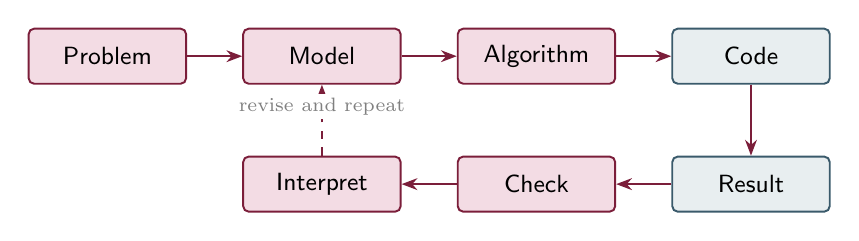
\begin{tikzpicture}[node distance=5mm and 7mm]
    \node[cycstep]                    (prob) {Problem};
    \node[cycstep, right=of prob]     (mod)  {Model};
    \node[cycstep, right=of mod]      (alg)  {Algorithm};
    \node[cycdo,   right=of alg]      (code) {Code};
    \node[cycdo,   below=9mm of code] (res)  {Result};
    \node[cycstep, left=of res]       (chk)  {Check};
    \node[cycstep, left=of chk]       (intp) {Interpret};
    \draw[flow] (prob) -- (mod);
    \draw[flow] (mod)  -- (alg);
    \draw[flow] (alg)  -- (code);
    \draw[flow] (code) -- (res);
    \draw[flow] (res)  -- (chk);
    \draw[flow] (chk)  -- (intp);
    \draw[flow, dashed] (intp.north) -- node[font=\scriptsize, text=Gray, fill=white, inner sep=1.5pt, above, pos=0.5]
          {revise and repeat} (mod.south);
\end{tikzpicture}%
}
%~~~~~~~~~~~~~~~~~~~~~~~~~~~~~~~~~~~~~~~~~~~~~~~~~~~~~~~~~~~~~~~~~~~~~~~~~~~~~~

%%%%%%%%%%%%%%%%%%%%%%%%%%%%%%%%%%%
%% SECTION SEPARATOR (ToC recap) %%
%%%%%%%%%%%%%%%%%%%%%%%%%%%%%%%%%%%
\AtBeginSection[]
{
{
    \setbeamercolor{background canvas}{bg=primaryLight!6}
    \begin{frame}[plain]
        \frametitle{Table of Contents}
        \tableofcontents[currentsection]
    \end{frame}
}
}
%%%%%%%%%%%%%%%%%%%%%%%%%%%%%%%%%%%

%~~~~~~~~~~~~~~~~~~~~~~~~~~~~~~~~~~~~~~~~~~~~~~~~~~~~~~~~~~~~~~~~~~~~~~~~~~~~~~
% Information
\title{Engineering Mini-Projects}
\subtitle{\emph{Engineering Computation with Python} --- Chapter 16}
\author{Mun\'{i}m Zabidi}
\institute{\color{primary}Faculty of Electrical Engineering, Universiti Teknologi Malaysia}
\date{\today}
\titlegraphic{assets/logoutmwhite.png}
%~~~~~~~~~~~~~~~~~~~~~~~~~~~~~~~~~~~~~~~~~~~~~~~~~~~~~~~~~~~~~~~~~~~~~~~~~~~~~~

\begin{document}

\titlepage

\begin{frame}{Table of Contents}
    \tableofcontents
\end{frame}

\begin{frame}{About These Projects}
    \leavevmode
    Every chapter of this course taught \alert{one technique at a time}.
    Real engineering problems do not arrive sorted by technique: a single
    question usually needs loading data, plotting it, cleaning it,
    fitting a model, and interpreting the result --- all at once.

    \vspace{2mm}
    The eight projects ahead are deliberately small, but each combines
    several chapters. None has a single correct program; what matters is
    that the answer is \alert{right}, that you can \alert{justify} it,
    and that you have \alert{checked} it.

    \vspace{2mm}
    \begin{alertblock}{Work through the full cycle for every project}
        Do not skip the checks --- a result you have not verified is not
        yet an answer.
    \end{alertblock}
\end{frame}

\begin{frame}{The Engineering Computation Cycle, Once More}
    \leavevmode
    \begin{center}
    \computationcycle
    \end{center}

    \vspace{2mm}
    {\small Each project below ends with a short list of checks --- a
    units check, a magnitude check, and an interpretation question. Use
    them the same way you have all course.}
\end{frame}

%===============================================================================
\section{Circuits: RC, RLC, and a Three-Loop Solver}
%===============================================================================

\begin{frame}{Project 1: RC Circuit Explorer}
    \leavevmode
    \textbf{Chapters used:} Plotting, Arrays, Units.

    \vspace{2mm}
    A capacitor $C$ charges through a resistor $R$ from a supply $V_0$:
    \[
    v_C(t) = V_0\left(1 - e^{-t/\tau}\right), \qquad \tau = RC .
    \]

    \vspace{2mm}
    Plot $v_C(t)$ for $R = 4.7\,\text{k}\Omega$, $C = 100\,\mu\text{F}$,
    $V_0 = 12\,\text{V}$, over $0$ to $5\tau$. Repeat on the same axes for
    $R = 1\,\text{k}\Omega$ and $R = 10\,\text{k}\Omega$. Describe what
    changing $R$ does to the shape.
\end{frame}

\begin{frame}{Project 1: Checks}
    \leavevmode
    \begin{block}{Units}
        $R$ in ohms times $C$ in farads gives $\tau$ in seconds. Here
        $\tau = 0.47\,\text{s}$.
    \end{block}

    \vspace{2mm}
    \begin{block}{Limiting case}
        At $t = \tau$, voltage should reach about $63\%$ of $V_0$,
        roughly $7.6\,\text{V}$. At $t = 5\tau$, within $1\%$ of $V_0$.
    \end{block}

    \vspace{2mm}
    \begin{alertblock}{Interpret}
        Does a larger $R$ make the capacitor charge faster or slower?
        Explain \alert{physically}, not just from the graph.
    \end{alertblock}
\end{frame}

\begin{frame}{Project 2: RLC Frequency Response}
    \leavevmode
    \textbf{Chapters used:} Complex impedance, Log plots.

    \vspace{2mm}
    Series RLC circuit: $R = 40\,\Omega$, $L = 0.2\,\text{H}$,
    $C = 50\,\mu\text{F}$.
    \[
    Z(f) = R + j\omega L - \frac{j}{\omega C}, \qquad \omega = 2\pi f.
    \]

    \vspace{2mm}
    Compute $Z(f)$ from $1\,\text{Hz}$ to $1\,\text{kHz}$. Plot
    $|Z|$ and phase $\theta$ against frequency on a \alert{logarithmic}
    frequency axis. Identify the resonant frequency from your plots.
\end{frame}

\begin{frame}{Project 2: Checks}
    \leavevmode
    \begin{block}{Theory}
        Resonance occurs when $X_L = X_C$, giving
        $f_0 = 1/(2\pi\sqrt{LC}) \approx 50.3\,\text{Hz}$. Does your
        magnitude plot reach its minimum there?
    \end{block}

    \vspace{2mm}
    \begin{block}{Magnitude}
        At resonance, $|Z|$ should fall to approximately
        $R = 40\,\Omega$, and the phase should cross zero.
    \end{block}

    \vspace{2mm}
    \begin{alertblock}{Interpret}
        Well below resonance the circuit is capacitive (negative phase);
        well above it is inductive. Confirm this from your phase plot.
    \end{alertblock}
\end{frame}

\begin{frame}[fragile]{Project 6: Circuit Solver}
    \leavevmode
    \textbf{Chapters used:} Matrices, Files.

    \vspace{2mm}
    Extend the two-loop mesh solver to \alert{three loops}. Build the
    $3 \times 3$ coefficient matrix $\mathbf{A}$ and source vector
    $\mathbf{b}$ for resistors and sources of your own choosing, solve
    $\mathbf{A}\mathbf{x} = \mathbf{b}$ with \texttt{np.linalg.solve},
    and print all three loop currents in milliamps.

    \vspace{2mm}
\begin{lstlisting}
def solve_loops(A, b):
    return np.linalg.solve(A, b)   # works for any number of loops
\end{lstlisting}
\end{frame}

\begin{frame}{Project 6: Checks}
    \leavevmode
    \begin{block}{Substitution}
        Compute \texttt{A @ x} and confirm it reproduces \texttt{b}.
    \end{block}

    \vspace{2mm}
    \begin{block}{Magnitude}
        For a low-voltage supply and resistors of hundreds of ohms,
        currents should be in the milliamp range. Amps would signal a
        units or matrix-construction error.
    \end{block}

    \vspace{2mm}
    \begin{alertblock}{Interpret}
        If a computed current is negative, what does that mean about the
        direction you assumed for that loop?
    \end{alertblock}
\end{frame}

%===============================================================================
\section{Data: Calibration, Noise, and Prediction}
%===============================================================================

\begin{frame}{Project 3: Sensor Calibration}
    \leavevmode
    \textbf{Chapters used:} Curve fitting, Plotting.

    \vspace{2mm}
    A temperature sensor outputs a voltage. Calibration data:

    \begin{center}
    \small
    \begin{tabular}{@{}lcccccc@{}}
    \toprule
    Voltage (V) & 0.5 & 1.0 & 1.5 & 2.0 & 2.5 & 3.0 \\
    Temp.\ (\textcelsius) & $-2.1$ & 12.4 & 27.0 & 41.8 & 56.2 & 70.9 \\
    \bottomrule
    \end{tabular}
    \end{center}

    \vspace{2mm}
    Fit $T = mV + c$ with \texttt{np.polyfit}, print the equation, plot
    the data with the fitted line, and compute the residual at each
    point. Convert a new reading of $1.75\,\text{V}$ to temperature.
\end{frame}

\begin{frame}{Project 3: Checks}
    \leavevmode
    \begin{block}{Fit}
        Should give approximately $T = 29.2V - 16.8$.
    \end{block}

    \vspace{2mm}
    \begin{block}{Residuals}
        All small (under $0.2\,^{\circ}\text{C}$), no systematic
        pattern. A \alert{curved} residual pattern would mean a straight
        line is the wrong model.
    \end{block}

    \vspace{2mm}
    \begin{alertblock}{Interpret}
        What does slope $m$ mean physically, in degrees per volt? What
        does intercept $c$ represent?
    \end{alertblock}
\end{frame}

\begin{frame}{Project 4: Noisy Signal Analysis}
    \leavevmode
    \textbf{Chapters used:} Arrays, Statistics, Plotting.

    \vspace{2mm}
    Generate a noisy $100\,\text{Hz}$ sine wave over two cycles:
    \[
    x(t) = \sin(2\pi f t) + n(t),
    \]
    with $n(t)$ from \texttt{np.random.normal}, standard deviation
    $0.3$. Plot the noisy signal, compute its mean and standard
    deviation, then threshold: set every sample whose magnitude is
    below $0.5$ to zero. Plot the result alongside the original.
\end{frame}

\begin{frame}{Project 4: Checks}
    \leavevmode
    \begin{block}{Magnitude}
        The mean of the noisy sine should be close to zero --- a full
        number of cycles of a sine averages out.
    \end{block}

    \vspace{3mm}
    \begin{alertblock}{Interpret}
        Thresholding removed small values --- but did it remove only
        noise? Examine what happened near the \alert{zero-crossings} of
        the sine, where the true signal is also small. What does this
        tell you about the limits of naive filtering?
    \end{alertblock}
\end{frame}

\begin{frame}{Project 7: A Simple Engineering Predictor}
    \leavevmode
    \textbf{Chapters used:} Machine learning, Statistics.

    \vspace{2mm}
    Using a small dataset relating motor operating current and ambient
    temperature to motor body temperature (plausible data, or your own
    measurements), train a \alert{linear regression} model with
    scikit-learn to predict motor temperature from the other two
    variables.

    \vspace{2mm}
    Split the data into training and testing sets, fit the model, and
    report its accuracy on the test set.
\end{frame}

\begin{frame}{Project 7: Checks}
    \leavevmode
    \begin{block}{Evaluation}
        Evaluate on the test split, \alert{never} on the training data.
    \end{block}

    \vspace{2mm}
    \begin{block}{Magnitude}
        Predicted temperatures should be physically plausible. A
        prediction of $-40\,^{\circ}\text{C}$ or $500\,^{\circ}\text{C}$
        signals a problem with the data or the model.
    \end{block}

    \vspace{2mm}
    \begin{alertblock}{Interpret}
        Does the model say higher current raises motor temperature? Does
        that match the physics you expect? Distrust a model whose
        coefficients contradict physical reasoning, even if its accuracy
        looks good.
    \end{alertblock}
\end{frame}

%===============================================================================
\section{Capstones: Energy and the Complete Bench Analysis}
%===============================================================================

\begin{frame}{Project 5: Battery Discharge}
    \leavevmode
    \textbf{Chapters used:} Differentiation/integration, Files.

    \vspace{2mm}
    A battery under a constant $0.5\,\text{A}$ load is logged once per
    minute for one hour; terminal voltage falls approximately linearly
    from $12.6\,\text{V}$ to $11.2\,\text{V}$.

    \vspace{2mm}
    \begin{enumerate}
        \item Plot voltage against time.
        \item Compute $dv/dt$ with \texttt{np.gradient}.
        \item Compute delivered energy $E = \int v\,i\,dt$ with
              \texttt{np.trapz}, converted to watt-hours.
    \end{enumerate}
\end{frame}

\begin{frame}{Project 5: Checks}
    \leavevmode
    \begin{block}{Units}
        Volts $\times$ amps $\times$ seconds gives joules; divide by
        $3600$ for watt-hours.
    \end{block}

    \vspace{2mm}
    \begin{block}{Magnitude}
        Energy should be roughly $5.9\,\text{Wh}$. Hand check: average
        voltage $11.9\,\text{V}$ $\times$ $0.5\,\text{A}$ $\times$ one
        hour $\approx 6\,\text{Wh}$ --- agrees.
    \end{block}

    \vspace{2mm}
    \begin{alertblock}{Interpret}
        $dv/dt$ is negative and roughly constant. What would a sudden
        \alert{steepening} of that slope indicate about the battery?
    \end{alertblock}
\end{frame}

\begin{frame}{Project 8: The Complete Bench Analysis}
    \leavevmode
    \textbf{Chapters used:} nearly all of them.

    \vspace{2mm}
    Return to \texttt{bench\_rc.csv}, the recurring dataset from the
    start of the course, and carry out the whole workflow yourself:

    \vspace{1mm}
    \begin{enumerate}\itemsep1pt
        \item Load the file; inspect shape and columns.
        \item Plot voltage against time.
        \item Repair the three missing samples near $t = 0.8\,\text{s}$
              by interpolation.
        \item Detect the corrupted temperature reading with the IQR
              rule, and replace it.
        \item Fit the discharge for the measured time constant.
        \item Differentiate the repaired voltage to estimate current
              from $i = -C\,dv/dt$; compare against the recorded column.
        \item Report measured $\tau$, nominal $\tau = RC = 0.47\,\text{s}$,
              and the percentage error.
    \end{enumerate}
\end{frame}

\begin{frame}{Project 8: A Hint and the Checks}
    \leavevmode
    \begin{block}{Hint}
        Taking the natural logarithm of $v(t) = V_0 e^{-t/\tau}$ gives a
        straight line whose slope is $-1/\tau$, so \texttt{np.polyfit}
        on \texttt{np.log(v)} versus \texttt{t} works directly.
    \end{block}

    \vspace{2mm}
    \begin{block}{Magnitude}
        Fitted $\tau$ should come out near $0.47\,\text{s}$ --- within a
        few percent is a good result for noisy measurements. The
        differentiated current will be noisier than the recorded
        column; differentiation amplifies noise.
    \end{block}

    \vspace{2mm}
    \begin{alertblock}{Interpret}
        Which current figure would you trust more for a report --- the
        measured column, or the one derived from the voltage? Justify
        your choice.
    \end{alertblock}
\end{frame}

\begin{frame}{A Closing Thought}
    \leavevmode
    \begin{center}
    \large
    If you can complete Project 8 unaided, you have done what this
    course set out to teach.
    \end{center}

    \vspace{4mm}
    \begin{block}{What that means}
        You have taken a real engineering measurement, expressed the
        physics mathematically, translated that mathematics into Python,
        computed a result, checked it, and interpreted what it means.
    \end{block}

    \vspace{4mm}
    \begin{center}
        \Large\color{primary}\textbf{That is engineering computation.}
    \end{center}
\end{frame}

\end{document}
